\documentclass[pdflatex,compress,mathserif]{beamer}

%\usetheme[dark,framenumber,totalframenumber]{ElektroITK}
\usetheme[darktitle,framenumber,totalframenumber]{ElektroITK}

\usepackage[utf8]{inputenc}
\usepackage[T1]{fontenc}
\usepackage{lmodern}
\usepackage[bahasai]{babel}
\usepackage{amsmath}
\usepackage{amsfonts}
\usepackage{amssymb}
\usepackage{graphicx}
\usepackage{multicol}
\usepackage{lipsum}
\usefonttheme[onlymath]{serif}

\newcommand*{\Scale}[2][4]{\scalebox{#1}{$#2$}}%

\setbeamertemplate{caption}[numbered]

\title{MATEMATIKA DASAR}
\subtitle{Persamaan Linear dan Kuadratik}

\author{Mifta Nur Farid}

\begin{document}

\maketitle

\section{Persamaan Linear dan Kuadratik}

\subsection{Persamaan}

\begin{frame}
\frametitle{Persamaan}
	\begin{itemize}
		\item Secara umum suatu persamaan adalah pernyataan dari dua buah ekspresi matematika yang bernilai sama.
		$$ 4 + 3 = 2 + 5 $$
		\item Dalam permasalahan yang akan dipelajari lebih lanjut akan mengandung suatu variabel, yang bisa dinyatakan dalam suatu simbol (biasanya dalam huruf) yang menyatakan suatu bilangan.
		$$ 4x+6 = 18 $$
		\item Nilai $x$ yang memenuhi persamaan tersebut disebut solusi atau akar dari persamaan.
	\end{itemize}
\end{frame}

\begin{frame}
	\frametitle{Persamaan}
	\begin{center}
		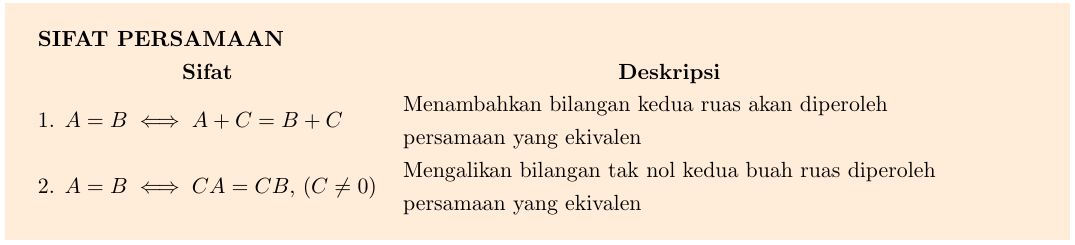
\includegraphics[width=\linewidth]{img/img01}
	\end{center}
\end{frame}

\end{document}
